\section{Обґрунтування системи параметрів ПП}
На підставі даних про основні функції, що повинен реалізувати програмний продукт, вимог до нього, визначаються основні параметри виробу, що будуть використані для розрахунку коефіцієнта технічного рівня.

\subsection{Опис параметрів}

Для того, щоб охарактеризувати програмний продукт, будемо використовувати наступні параметри:
\begin{description}
	\item[$X_1$] - швидкодія мови програмування;
	\item[$X_2$] - об’єм пам’яті для збереження даних;
	\item[$X_3$] - час обробки даних;
	\item[$X_4$] - потенційний об’єм програмного коду.
\end{description}

$X_1$ відображає швидкодію операцій залежно від обраної мови програмування. 

$X_2$ відображає об'єм оперативної пам'яті персонального комп'ютера, що необхідний для збереження та обробки даних під час виконання програми.

$X_3$ відображає час, який витрачається на дії.

$X_4$ показує кількість програмного коду який необхідно створити безпосередньо розробнику. 

\subsection{Кількісна оцінка параметрів}
Гірші, середні і кращі значення параметрів вибираються на основі вимог замовника й умов, що характеризують експлуатацію ПП як показано у табл.~\ref*{tab:economics_program_parameters}

\begin{table}[H]
	\caption{Основні параметри ПП}
	\centering
\begin{tabular}{|p{0.3\textwidth}|p{0.11\textwidth}|p{0.1\textwidth}|p{0.1\textwidth}|p{0.1\textwidth}|p{0.1\textwidth}|}
	\hline
	Назва параметра & Умовні позначення & Одиниці виміру & \multicolumn{3}{c|}{Значення параметра} \\ \cline{4-6}
	& & & гірші & середні & кращі \\
	\hline	
	Швидкодія мови програмування & $X_1$ & оп/мс & 19000 & 11000 & 2000 \\ 
	\hline
	Об'єм оперативної пам'яті & $X_2$ & мб & 32 & 16 & 8 \\
	\hline
	Час обробки зображення & $X_3$ & мс & 1000 & 420 & 60  \\
	\hline
	Об'єм програмного коду & $X_4$ & строк & 2000 &1500& 1000 \\
	\hline
\end{tabular}		
	\label{tab:economics_program_parameters}
\end{table}

За даними таблиці \ref{tab:economics_program_parameters} будуються графічні характеристики параметрів: рис.~\ref{fig:economics:x1} - рис.~\ref{fig:economics:x4} 
%TODO

\begin{figure}
	\centering
	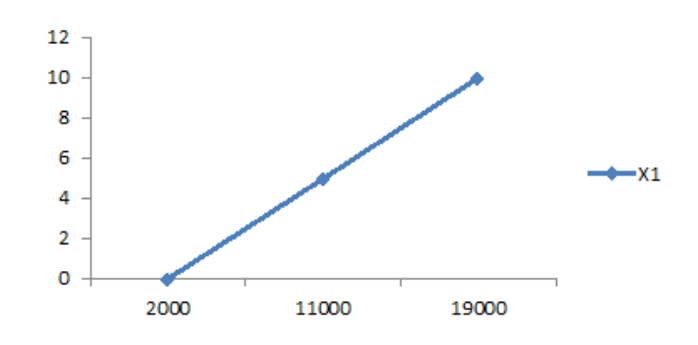
\includegraphics[width=0.7\linewidth]{economics/img/x1}
	\caption{Швидкодія мови програмування $X_1$}
	\label{fig:economics:x1}
\end{figure}
\begin{figure}
	\centering
	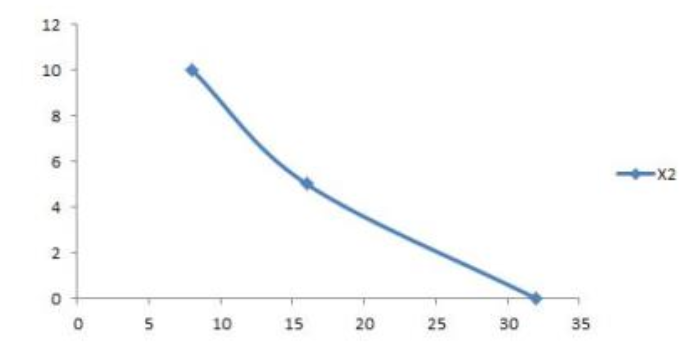
\includegraphics[width=0.7\linewidth]{economics/img/x2}
	\caption{Об'єм оперативної пам'яті $X_2$}
	\label{fig:economics:x2}
\end{figure}
\begin{figure}
	\centering
	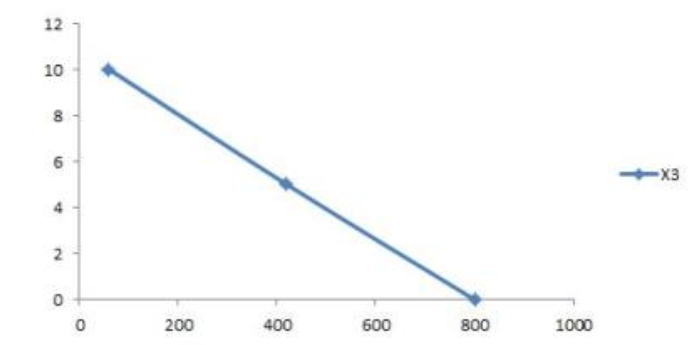
\includegraphics[width=0.7\linewidth]{economics/img/x3}
	\caption{Час, який витрачається на дії $X_3$}
	\label{fig:economics:x3}
\end{figure}
\begin{figure}
	\centering
	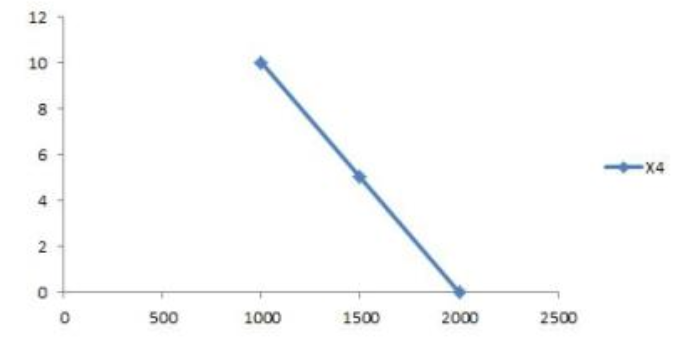
\includegraphics[width=0.7\linewidth]{economics/img/x4}
	\caption{Об'єм програмного коду $X_4$}
	\label{fig:economics:x4}
\end{figure}

\subsection{Аналіз експертного оцінювання параметрів}
Після детального обговорення й аналізу кожний експерт оцінює ступінь важливості кожного 
параметру для конкретно поставленої цілі – розробка програмного продукту, який дає найбільш 
точні результати при оптичному аналізі нотних листів.

Значимість кожного параметра визначається методом попарного порівняння. Оцінку проводить експертна комісія із 7 людей. Визначення коефіцієнтів значимості передбачає: 
\begin{itemize}
	\item визначення рівня значимості параметра шляхом присвоєння різних рангів; 
	\item перевірку придатності експертних оцінок для подальшого використання; 
	\item визначення оцінки попарного пріоритету параметрів; 
	\item обробку результатів та визначення коефіцієнту значимості. 
\end{itemize}

Результати експертного ранжування наведені у таблиці~\ref{tab:economics:parameter_range}.

\begin{table}[H]
	\caption{Результати експертного ранжування параметрів}
	\centering
	\begin{tabular}{| m{0.08\textwidth} | p{0.2\textwidth} | m{0.02\textwidth} | m{0.02\textwidth} | m{0.02\textwidth} | m{0.02\textwidth} | m{0.02\textwidth} | m{0.02\textwidth} | m{0.02\textwidth} |	p{0.08\textwidth}|p{0.08\textwidth}|p{0.09\textwidth}|}
	\hline
	\multirow{2}{*}{\rotatebox{90}{Позначення  }} & Назва & \multicolumn{7}{c|}{\parbox[c]{0.3\textwidth}{Ранг за оцінкою\\експерта}} 	& Сума рангів $R_i$ & Відх. $\Delta$ &$\Delta^2 $ \\
	\cline{3-9}
			   & 	   & 1& 2& 3& 4& 5& 6& 7							&					&					&\\ 
	\hline
	$X_1$, оп/мс & Швидкодія мови програмування 	& 4& 3& 4& 4& 4& 4& 4& 27& 0.75 	& 0.56 \\
	\hline
	$X_2$, мб	& Об'єм оперативної пам'яті 	& 4& 4& 4& 3& 4& 3& 3& 25&-1.25	& 1.56 \\ 
	\hline
	$X_3$, мс	& Час, який витрачається на дії		& 2& 2& 1& 2& 1& 2& 2& 12&-14.25& 203.06\\
	\hline
	$X_4$, строк & Об'єм програмного коду		& 5& 6& 6& 6& 6& 6& 6& 41& 14.75& 217.56\\
	\hline
	Разом		& 								&15&15&15&15&15&15&15& 105 & 0 & 420.75\\
	\hline
	\end{tabular}
	\label{tab:economics:parameter_range}
\end{table}

Для перевірки степені достовірності експертних оцінок, визначимо наступні параметри: 
\begin{enumerate}
	\item сума рангів кожного з параметрів і загальна сума рангів:
	\begin{equation}
		R = \sum\limits_{i=1}^{n} R_i = \cfrac{Nn(n+1)}{2} = 105 
	\end{equation}
	де $n$ - число оцінюваних параметрів, $N$ - число експертів
	
	\item середня сума рангів:
	\begin{equation}
		T = \cfrac 1n \sum\limits_{i,j} R_{ij} = 24.5
	\end{equation}
	
	\item відхилення суми рангів кожного параметра від середньої суми рангів:
	\begin{equation}
		\Delta_i = R_i - T \qquad i=1\ldots n
	\end{equation}
	Сума відхилень по всім параметрам повинна дорівнювати $0$;
	
	\item загальна сума квадратів відхилення:
	\begin{equation}
		S = \sum\limits_{i=1}^{N} \Delta^2 = 35
	\end{equation}
\end{enumerate}

Порахуємо коефіцієнт узгодженості: 
\begin{equation}
	W = \cfrac{12\cdot S}{N^2(n^3-n)}
\end{equation}
Ранжування можна вважати достовірним, тому що знайдений коефіцієнт узгодженості перевищує нормативний, котрий дорівнює $0.67$.

Скориставшись результатами ранжування, проведемо попарне порівняння всіх параметрів і результати занесемо у таблицю~\ref{tab:economics:pair_wise_eval}
\begin{table}[H]
	\caption{Попарне порівняння параметрів}
	\centering
	\begin{tabular}{| p{0.2\textwidth} | p{0.02\textwidth} | p{0.02\textwidth} | p{0.02\textwidth} | p{0.02\textwidth} | p{0.02\textwidth} | p{0.02\textwidth} | p{0.02\textwidth} | p{0.14\textwidth}|p{0.14\textwidth}|}
	\hline
	Параметри	& \multicolumn{7}{c|}{Експерти} & Кінцева оцінка & Чисельне значення \\
	\cline{2-8}
				& 1 & 2 & 3 & 4 & 5 & 6 & 7		&				& \\
	\hline
	X1 і X2 &=& >& =& <& =& <& <& < & 0.5 \\
	\hline
	X1 і X3 &< &< &< &< &< &< &< &< & 0.5\\
	\hline	
	X1 і X4 &> &> &> &> &> &> &> &> & 1.5\\
	\hline	
	X2 і X3 &< &< &< &< &< &< &< &< & 0.5\\
	\hline	
	X2 і X4 &> &> &> &> &> &> &> &> & 1.5\\
	\hline	
	X3 і X4 &> &> &> &> &> &> &> &>	 & 1.5 \\
	\hline	
	\end{tabular}
	\label{tab:economics:pair_wise_eval}
\end{table}

Числове значення, що визначає ступінь переваги $i$–го параметра над $j$–тим, $a_{ij}$ визначається по формулі: 
\begin{equation}
	a_{ij} = 
	\left\lbrace 
	\begin{array}{cc}
		1.5 ,&\quad X_i > X_j \\
		1.0 ,&\quad X_i = X_j \\
		0.5 ,&\quad X_i < X_j
	\end{array} 
	\right. 
\end{equation}
З отриманих оцінок складемо матрицю $ A = || a_{ij} || $

\newcommand{\weightcoef}[1]{K_\text{в}^{(#1)}}
Для кожного параметра зробимо розрахунок вагомості $ \weightcoef{i} $ за наступною формулою: 
\begin{equation}
	\weightcoef{i} = \cfrac{b_i}{\sum_{j=1}^n b_j} \quad ,\text{де} \quad b_i = \sum_{j=1}^n a_{ij}
\end{equation}

Відносні оцінки розраховуються декілька разів доти, поки наступні значення не будуть незначно відрізнятися від попередніх (менше $2\%$).На другому і наступних кроках відносні оцінки розраховуються за наступними формулами:

\begin{equation}
	\weightcoef{i} = \cfrac{b'_i}{\sum_{j=1}^n b'_j} \quad ,\text{де} \quad b'_i = \sum_{j=1}^n a_{ij}\cdot b_j
\end{equation}

Як видно з таблиці~\ref{tab:economics:weight_param}, різниця значень коефіцієнтів вагомості не перевищує $2\%$, тому більшої кількості ітерацій не потрібно.

\begin{table}[ht]
	\centering
	\caption{Розрахунок вагомості параметрів}
\begin{tabular}{| p{0.17\textwidth} | p{0.033\textwidth} | p{0.033\textwidth} | p{0.033\textwidth} | p{0.033\textwidth} | p{0.06\textwidth} | p{0.07\textwidth} | p{0.06\textwidth} | p{0.07\textwidth} |	p{0.06\textwidth}|p{0.07\textwidth}|}
	\hline
	\multicolumn{5}{|c|}{Ітерації} & \multicolumn{2}{c|}{1} & \multicolumn{2}{c|}{2} & \multicolumn{2}{c|}{3} \\
	\hline
	Параметри $X_i$ & $X_1$ & $X_2$ & $X_3$ & $X_4$ &
	 $b_i$ & $\weightcoef{i}$ & $b_i^1$ & $\weightcoef{i}$ & $b_i^2$ & $\weightcoef{i}$\\
	\hline
	 $X_1$ &1.0 &0.5 &0.5 &1.5 &3.5& 0.219 &22.25 &0.216 &100& 0.215 \\
	\hline
	 $X_2$ &1.5& 1.0& 0.5& 1.5& 4.5& 0.281& 27.25& 0.282& 124.3& 0.283\\
	\hline
	 $X_3$ &1.5& 1.5& 1.0& 1.5& 5.5& 0.344& 34.25& 0.347& 156& 0.348\\
	\hline	 
	 $X_4$ &0.5& 0.5& 0.5& 1.0& 2.5& 0.156& 14.25& 0.155& 64.75& 0.154\\
	\hline	 
	\multicolumn{5}{|l|}{Всього:} &16 &1 &98 &1 &445 &1 \\
	\hline
\end{tabular}	
	\label{tab:economics:weight_param}
\end{table}